
\chapter{Results: Model's properties and individuals response}
%(Related to the notions cited above, like performance decomposition)


\section{Parameter filtering and sensitivity analysis}
Obj: give confidence in the model, demonstrate is able to reproduce simple growth pattern.\\
Obj2: have a beter idea of plasticity effect on growth.
growth plastic and non plastic parameter filtering: can we distinguish species thanks to species specific parameters instead of shared parameters.\\
does plasticity make it easier ?\\
Impact of plasticity related parameters.\\

\subsection{Method}

\paragraph{Pot data}
Pot data consists in total biomass and root shoot ration (RSR) data of ... species grown in pots by Peterson and al. (peterson). This old dataset has the advantages of being grass species grown in a described steady environment with two conditions of watering with measures of essential components of growth: biomass and RSR. The inputs used to simulated these experriment are detailed in appendix.

\paragraph{Individual calibration process}
Bayessian calibration could not be used for the model considering the number of parameters and the simulation time. A filtering process has been implemented in R. Parameters are sampled following the LHS method (from \texttt{lhs} package)	within parameter ranges (desccribed in table ...) defined from the litterature, and constraints dicted by desired behaviours from the model. When necessary the sample is log transformed. Because of strong relationship between exchange rate parameters and cost of exchagne area, exchanges rates parameters are expressed on a mass basis for sampling then transform to an area basis for the model. Phtosynthetic activity is defined relatively to the water uptake activity and water use efficiency (WUE) to avoid extreme root shoot ratios.\\

Once generated a first filtering is applied to save simulation time and avoid unrealistic trait values (see table for ranges extracted from LES data in alpine biome) that are not tested against calibartion data.\\
Once the parameters transformed and filtered, simulations matching growth conditions in Peterson experiments.\\
Generated data from finished simulations (i.e. plant lives until the end and do not exceed model's internal size limits) are then compared to experiment data species by species. Parameters of logistic distribution are computed from species means and standards deviantions for RSR and total biomass. The use of this distribution form is justified by the intrinsic form of RSR measure and the need to reject negative values for total biomass. A parameter set is accepted for one species if it within a 95\% range of the calculated distribution for both RSR and total biomass in wet and dry conditions.\\



\subsection{Results}


\paragraph{Individual calibration}. Calibration filtering results in the selection of n parameter sets over m preselected parameters sets. Accepted sets are distributed among the 11 species of the dataset like presented in the table. Species A, B and C are the most numerous.\\
sensitivity analysis. The models about seems to be sensitive to the following parameters: $r_1$, $\beta_0$, $P_{max}$, $u_{max}$, $k_{or}$, $\rho_{ar}$. The four first parameters are related to global resource availability and directly related to growth rate, while the second and the last three and related to the below-ground resource foraging and exchange rate.\\
Total biomass is particularly sensitive to exchange rate parameters, but also tissue construction cost. (not shown)\\

Plasticity does not change the acceptance rate in any form (only slight increased from 0.26\% to 0.38\%). Despite non overlapping (around respectively and third and a quarter of accepted parameter sets are shared between non plastic and plastic calibration) the distribution of not shared parameter sets are very similar and does not show any clear pattern. \\

\begin{figure}
%\includegraphics[width = \textwidth]{/mnt/quadri1/simulations/exploration/species_par_space2017-10-26/plots/acceptance_rate_RSRnWeight_per_par.pdf}
\caption{Acceptance rate per parameter for individual growth. No plasticity}
\end{figure}

\begin{figure}
%\includegraphics[width = \textwidth]{/mnt/quadri1/simulations/exploration/species_par_space2017-11-06/plots/acceptance_rate_RSRnWeight_per_par.pdf}
\caption{Acceptance rate per parameter for individual growth. RSR plasticity}
\end{figure}

Acceptance rate without plasticity:
% latex table generated in R 3.2.3 by xtable 1.8-2 package
% Wed Nov 15 13:36:59 2017
\begin{table}[ht]
\centering
\begin{tabular}{rlrr}
  \hline
 & species & nb accepted & rate \\ 
  \hline
1 & Silene acaulis & 227 & 0.02 \\ 
  2 & Trifolium dasyphyllum & 271 & 0.03 \\ 
  3 & Geum rossii & 51 & 0.01 \\ 
  4 & Thlaspi alpestre & 342 & 0.03 \\ 
  5 & Deschampsia caespitosa & 0 & 0.00 \\ 
  6 & Eriogonum umbellatum & 500 & 0.05 \\ 
  7 & Townsendia scapigera & 593 & 0.06 \\ 
  8 & Astragalus whitneyi & 1570 & 0.16 \\ 
  9 & Lupinus lobbii & 678 & 0.07 \\ 
  10 & Erigeron peregrinus & 1 & 0.00 \\ 
  11 & Oxyria digyna & 0 & 0.00 \\ 
   \hline
\end{tabular}
\end{table}

Acceptance rate with RSR plasticity for equilibrium:
% latex table generated in R 3.2.3 by xtable 1.8-2 package
% Wed Nov 15 13:39:16 2017
\begin{table}[ht]
\centering
\begin{tabular}{rlrr}
  \hline
 & species & nb accepted & rate \\ 
  \hline
1 & Silene acaulis & 396 & 0.04 \\ 
  2 & Trifolium dasyphyllum & 317 & 0.03 \\ 
  3 & Geum rossii & 72 & 0.01 \\ 
  4 & Thlaspi alpestre & 360 & 0.04 \\ 
  5 & Deschampsia caespitosa & 0 & 0.00 \\ 
  6 & Eriogonum umbellatum & 805 & 0.08 \\ 
  7 & Townsendia scapigera & 930 & 0.09 \\ 
  8 & Astragalus whitneyi & 2424 & 0.24 \\ 
  9 & Lupinus lobbii & 868 & 0.09 \\ 
  10 & Erigeron peregrinus & 0 & 0.00 \\ 
  11 & Oxyria digyna & 0 & 0.00 \\ 
   \hline
\end{tabular}
\end{table}


Change of relationship between parameters and acceptance rate -> none\\
accept = f(tau)\\

PCA reveal that sensitive parameters are also the dominant variables in the main components of the component analysis of the accepted parameter sets. Species cannot be distinguished on the two main component space, neither on 1 or 2D species specific parameters space (l\_ini, w\_ini, w\_ini vs l\_ini, as\_s\_d, as\_r\_d, as\_r\_d vs as\_s\_d) despite small variations in distribution shapes between species.\\



\begin{figure}
%\includegraphics[width = 10cm]{/mnt/quadri1/simulations/exploration/species_par_space2017-11-06/plots/var_imp_plot_eq_design.pdf}
\caption{Importance of the random forest to explain filtering outcome (accepted or rejected) of a balanced sample of parameter set between all tested (all accepted parameters and an equivalent sample in rejected parameters).  RSR plasticity.}
\end{figure}

\begin{figure}
%\includegraphics[width = 10cm]{/mnt/quadri1/simulations/exploration/species_par_space2017-11-06/plots/PCA_acc.pdf}
\caption{Accepted parameters set for plastic individual growth calibration filtering  on the two main components of PCA.}
\end{figure}

\paragraph{Acceptance rate}
Rerun acceptance rate for non plastic simulations with growth only.

\paragraph{Sensitivity}

\paragraph{Root shoot ratio and plasticity}

\subsection{Discussion}

\paragraph{Growth and strategy space}

\textbf{Growth is reproduced, but only for one species, not full strategy space.}

\paragraph{}

\textbf{Sensitivity of different variable to the parameters make sense and align with the two criterion of selection (that work with the independence of trade-off).}

\paragraph{}

\textbf{Root shoot ratio changes were not captured by the model. The structure of the plasticity mechanisms does not work with the given watering cycle. Needs to add one parameter for reactivity.}


\section{Individual level behaviour and properties}
%Proof of concept
\subsection{Method}


\paragraph{Strategy diversity filtering}
To further reduce the number of parameter sets considered, we proceeded in an additional filtering step. Because the first filtering was conduced for only one strategy over the whole 4D strategy space (l\_ini,  w\_ini, as\_s\_d, as\_r\_d) it is necessary to verify that other strategies do not lead to potential Darwinian demon. This should be limited by the choice of priors, while at the same time promoted by the selection of parameters increasing growth to counter balance potential unfitted strategies\footnote{Better do that beforehand than after... But I guess it's too late now.}.

\paragraph{Simulation setup}
All common parameters for pot simulations. i.e. weather, soil, default species parameters.


\subsection{Results}


\subsection{Discussion}
\paragraph{Allocation rules, plasticity and performance}

\textbf{Allocation rules are extremely important as they reduce the phenotypic space explore. Without even considering plasticity. Need a good understanding of the performance within the phneotypic landscape. Plus there is a need for alignment between starting phenotype and endpoint. Will also affect how plasticity is driven.}

\paragraph{Fast slow strategy and allocation trade-off}

\textbf{Allocation trade-off allow for strategies from the fast-slow spectrum to arise, independently for shoot and root, in coherent framework. Potential effect of other strategy axis can be analysed alongside this trade-off, even if they affect composite traits like SLA or SRL.}

\paragraph{Memory and phenotypes}

\textbf{Memory is a strong enough driver to control plant organ strategy. The effect of overall activity should be studied too and considered if memory is used to determine the default phenotype.)}

\section{Performance landscape, plasticity and response to a gradient}

\subsection{Method}

\subsection{Results}


\subsection{Discussion}

\paragraph{Convergence to subspace}

Somehow I need to talk about the cost of being wrong. Can be observe in the delta heatmap on delta strat and delta w-ini: in this case there is less impact of being wrong of memory if you're good with strategy, because your not in different conditions...\\

\textbf{The phenotypic plasticity implemented in \model improve the relative performance of multiple strategies by concentrating the plant toward a subspace of higher performance for most of plants. Convergence to a smaller subspace can be assimilated to reduction in phenotypic diversity, but it reduce performance heterogeneity and should favour local plant diversity. Meta-community diversity is however reduces by the reduction of potential axis for niche differentiation. Plasticity costs and limits should play major role in the balance between these mechanisms. Community level simulations are needed to further understand the cumulative role of competition, spatial and temporal variability and plasticity costs on phenotypic plasticity influence on plant community dynamics.}

\paragraph{Improvement in variable conditions}

\textbf{Phenotypic plasticity }

\paragraph{Heterogeneity of response}

Kichenin (different response to gradient) Doesn't work in this framework: Not so sure about that: depending on your initial memory plants show directional changes toward one phenotype. Yeah, but they should have converged for other conditions too... So, it doesn't work. Might be explained by:
\begin{itemize}
\item different conditions: because heterogeneity and habitat selection, or changes in competition hierarchy;
\item different ways to tackle changes on one dimensions;
\item different weights between mechanisms impacting composite traits, because of the different traits.
\end{itemize}

% Use these notes to extend the discussion and add some outlooks
%
%\section{Niche response}
%
%
%Obj1: understand how resource use mechanisms and allocation algorithms shape the environmental potential niche in the context of the model.\\
%H1: strategy and memory affect niche in two ways if we suppose they are independent: shape and position. Strategy mostly affect shape (width and height) while memory (and so root:shoot ratio) affect mostly position.\\
%H1': there is strong link between strategy and memory in the case of optimisation allocation that increase niche height and might reduce its width.\\
%Obj2: understand the role of plasticity on the niche and if the effect in the same for all strategies/memories.\\
%H2: the plasticity increase niche width but not height (as phenotype is optimum at the center of the niche where memory match the resource availability).
%
%Stability and efficiency trade-off. Niche heigh and width and relationship with the strategy. How does plasticity affect that ? Does it increase the height and widen niches ? What does that mean for coexistence ?\\
%Hopefully higher niche would go with unstable niche.
%%
%%\section{Transitivity and competition}
%%1 vs 1 interactions\\
%%Is the resource competition transitive ? How does niche widening impact that, does plasticty change competition interaction. Is it related to the trait distance ? (don't think so)
